\documentclass[a4paper, 12pt, conference]{IEEEtran}
\special{papersize=210mm,297mm} % Fix compatibility issues. A4 dimensions hard coded.
\usepackage[a4paper, top=0.8in, bottom=0.8in, left=0.6in, right=0.6in]{geometry}
\usepackage[utf8]{inputenc}
\usepackage[pdftex]{color, graphicx}
\usepackage[official]{eurosym}
\usepackage{fancyhdr}
\usepackage{amsfonts}
\usepackage{amsmath}
\usepackage{amsthm}
\usepackage{amssymb}
\usepackage{tabularx, caption}
\usepackage{setspace}
\usepackage{soul} % Text highlighting
\usepackage{type1cm} % Scalable Computer Modern font support
\usepackage{verbatim}
\usepackage{hyperref} % Support for PDF Hyper References and links
\usepackage{lastpage} % To get number of pages
\usepackage{listings} % To include code blocks
\usepackage{color}
\usepackage[acronym]{glossaries}

\def\arraystretch{1.4}

\newcommand{\upsc}[1]{\textsc{#1}}
\loadglsentries{acronyms}  
\makeglossaries

\newcommand{\todo}[1]{}
\renewcommand{\todo}[1]{{\color{blue} TODO:  {#1}}}

\def \FIXME {{\parindent -60px \sethlcolor{red} \color{white} \texthl{\textbf{FIXME}} \sethlcolor{yellow} \hskip 5px}}
\def \redhl #1{\sethlcolor{red} {\color{yellow} \textbf{\texthl{#1}}} \sethlcolor{yellow}}
\def \sitat #1{\textsuperscript{\cite{#1}}}
\def \const #1{\penalty 100 \hbox{\texttt{#1}}}
\newcommand{\HRule}{\rule{\linewidth}{0.2mm}}



\hypersetup{
colorlinks,%
citecolor=black,%
filecolor=black,%
linkcolor=black,%
urlcolor=black%
}

\setlength{\headheight}{14pt}

\ifCLASSINFOpdf

\else

\fi

\hyphenation{op-tical net-works semi-conduc-tor}
\def \thetitle {Awesome graph database benchmark shit}
\def \thesubtitle {}
\def \theauthor {Helge Hoff, Kim Hartvedt Andreassen, Jon Foss Mikalsen}

%\pagestyle{fancy}
\pagestyle{fancyplain} % options: empty , plain , fancy
\renewcommand{\headrulewidth}{1pt} % customise the layout...
\renewcommand{\footrulewidth}{0pt}
\lhead{\fancyplain{}{\thetitle{} -- \thesubtitle{}}}\chead{}\rhead{\fancyplain{}{\theauthor{}}}
\lfoot{}\cfoot{Page {\thepage} of \pageref{LastPage}}\rfoot{}


\begin{document}
\title{\thetitle}
\author{\theauthor}

\maketitle
\thispagestyle{plain}

%ABSTRACT
%\begin{abstract}
%When written in 
%\end{abstract}
 
\IEEEpeerreviewmaketitle

\section{Introduction}

\section{Background}
Social network applications are becoming increasingly popular, and traditional SQL databases are not well-suited to store large social networks with relationships between users.
Representing relationships in SQL databases often results in inefficient table joins, degrading performance significantly.
 
\todo{Use citation, explain neo4j scaling(index-free-adjacency)}
\cite{neo_scale}
\section{Integration of ShareDrive}
\section{Benchmark}
The benchmark consisted of finding friendship relations between users within a social network.
Finding friends of a user, friends of friends an so on, for each increment the result set increases exponentially.
Such queries are typical for social network applications, such as Facebook or Twitter, and are processed in real time, therefore, performance is vital for user experience.
\todo{Explain figure, might change placement?}
\begin{figure}[h]
	\centering
	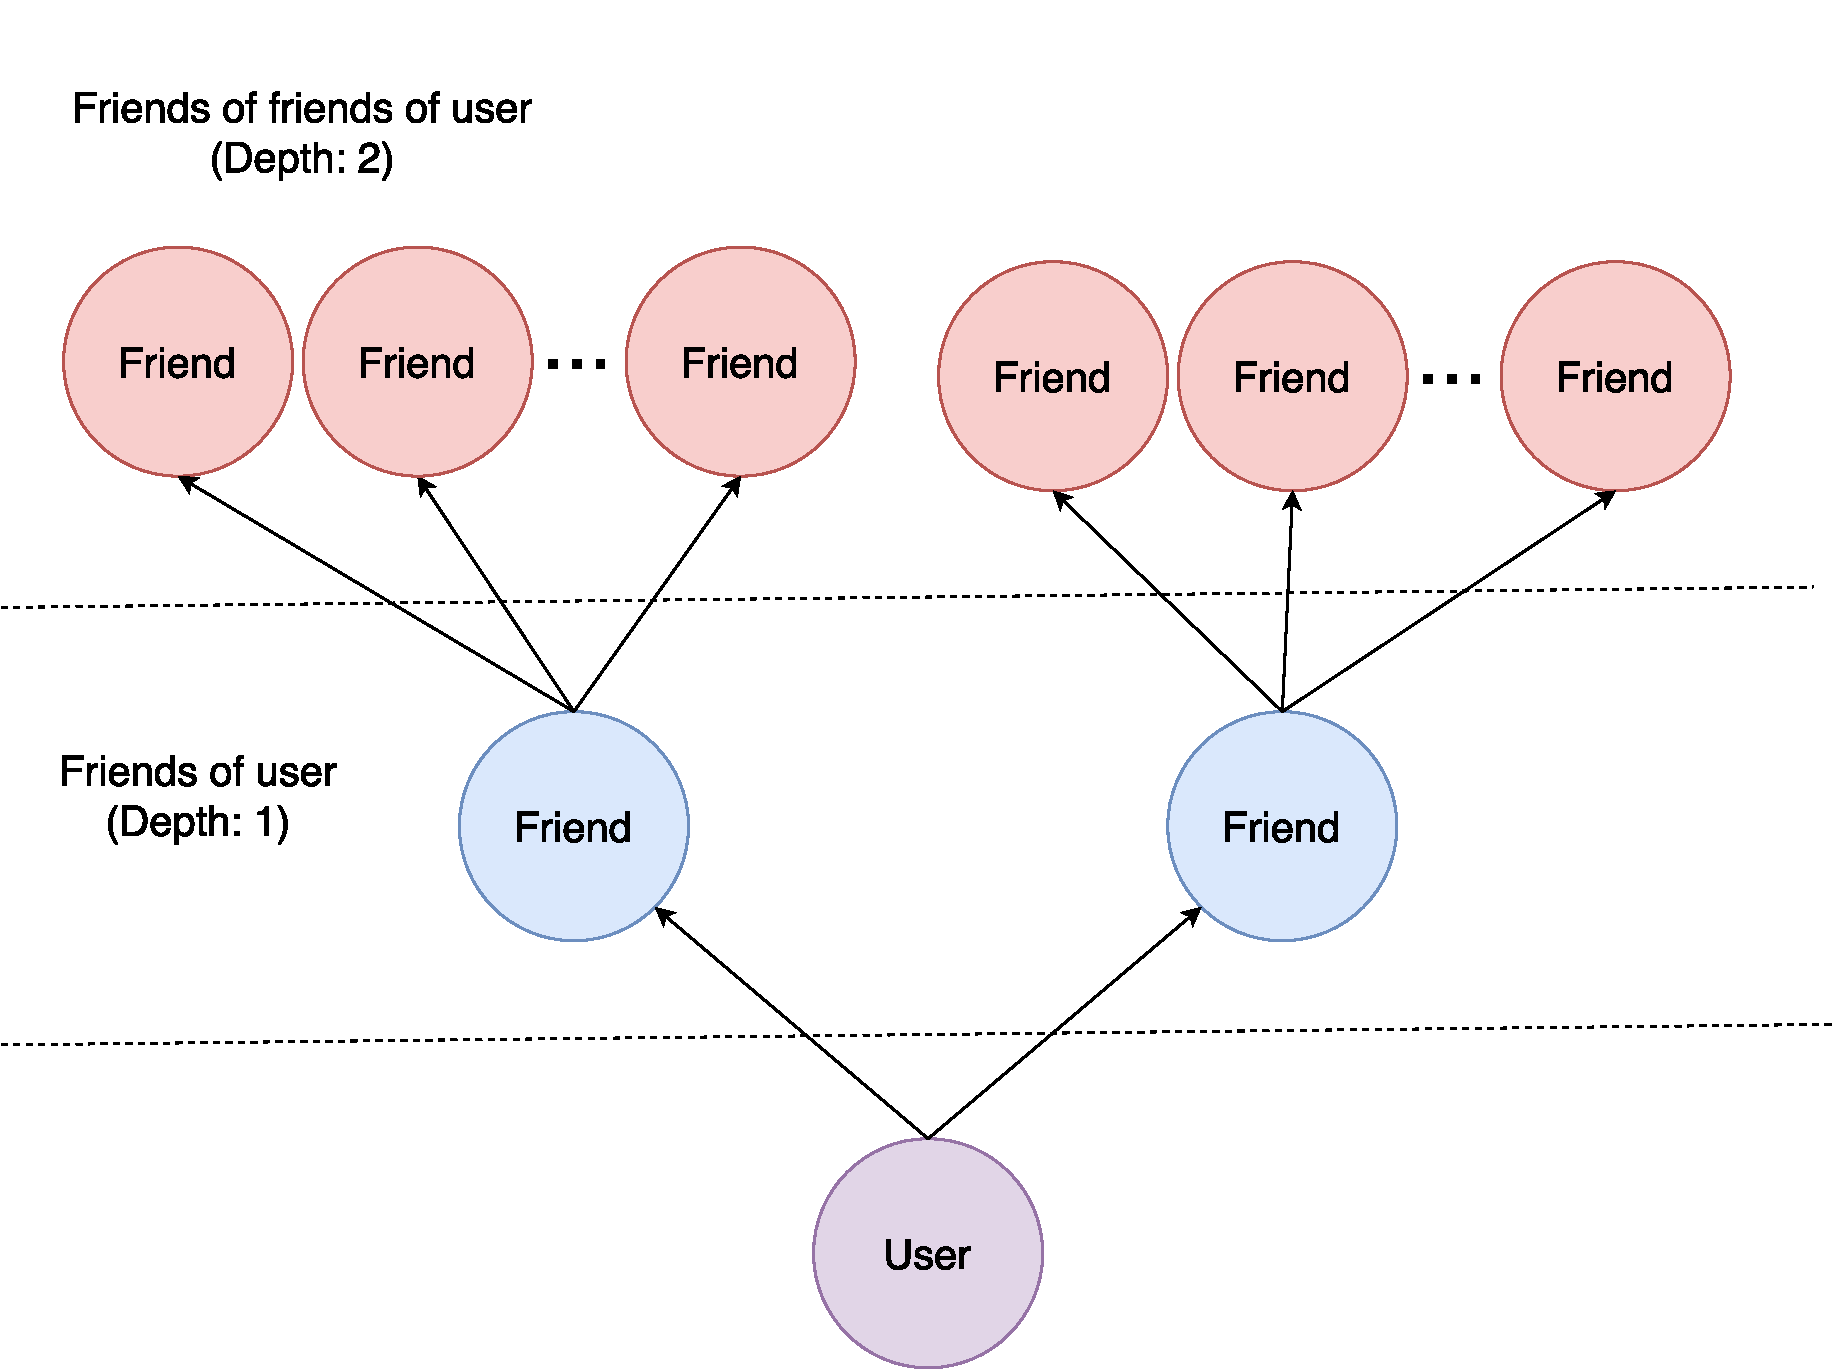
\includegraphics[scale=0.3]{friends.pdf}
	\caption{Query model for multi-level friendship queries.}
\end{figure}
\subsection{Experimental setup}
A dataset provided by Facebook, containing social circles, was used to conduct the experiment.
The dataset included several features describing anonymous Facebook users, however, for our experiment, only friendships between users were included.
Our test environment is as follows: 
\begin{itemize}
	\item Processor: Intel® Core™ i7-4500U CPU @ 1.80GHz.
	\item 8GB of memory. 
	\item Neo4j version: 3.1.2
	\item SQL database: MySQL 5.7.17
	\item Operating system: Ubuntu 16.04
\end{itemize}
On Facebook, friendships has to be mutual, hence, only requiring a one-way relationship, but for query simplicity they were represented as two-way relationships in the sql database.
%Friendships between users in the sql database was represented as a two-way relationship, mainly due to query simplicity.
\subsection{Discussion}
\todo{Explain result table etc}
\begin{table}[t]
	\centering
	\begin{tabular}{c|c|c}
		\textbf{Depth} & \textbf{Neo4j} (s) & \textbf{MySQL} (s) \\ \hline
		1 & 0.0238 & 0.0563 \\ \hline
		2 & 0.0366 & 0.147 \\ \hline
		3 & 0.143 & 3.136 \\ \hline
		4 & 0.378 & 94.001 \\
	\end{tabular}
	\caption{Performance comparison of multi-level friendship queries between Neo4j and MySQL. Query times are shown in seconds.}
\end{table}


\section{Conclusion}


%%% BIBLOGRAPHY

\newpage

\bibliographystyle{ieeetr}
\bibliography{sources}

\end{document}







